% Dokumentanklasse: a4paper, 14pt
% Beschreibung:     Dokumentenformat
% Option:           extraarticle - ?
\documentclass[12pt]{article}

% Paket:            showframe
% Beschreibung:     Blendet alle Frames (Textkörper, Fußzeile Kopzeile, Seitenrand) ein
% Option:
% \usepackage{showframe}

% Paket:            geometry
% Beschreibung:     A4 Seitenabstände
% Option:
\usepackage{geometry}
\geometry{
%  a4paper,           % Papierformat (wird auch über die Dokumentenklasse definiert)
  top=2.7cm,          % Abstand Kopfseite   (Zwischen Kopfseite und Inhalt)
  bottom=2cm,         % Abstand Fußseite    (Zwischen Fußseite und Inhalt)
  left=2.5cm,         % Abstand Linkeseite  (Zwischen Linkerseite und Inhalt)
  right=2cm,          % Abstand Rechteseite (Zwischen Recherseite und Inhalt)
%  width=              %                    textwidth (+marginsep +marinparwidth)
%  textwidth=15cm,     % Textbreite
%  marginparsep=1cm,   % Randnotiztrennng
%  marginparwidth=10cm,% Randnotizbreite
%  height=             %                    textheight (+headheight +headsep + footskip)
%  textheight=        % Texthöhe
  headheight=1cm,     % Kopfhöhe
  headsep=0.5cm,      % Kopftrennung        (Größe zwischen Kopfzeile und Inhalt)
  footskip=1cm,       % Fußzeilenhöhe
}

% Paket:            ansmath
% Beschreibung:     Zum darstellen von mathematischen Formeln
\usepackage{amsmath}

% Paket:            eurosym
% Beschreibung:     Bildet das Euro-Zeichen in unterschiedlichen Varianten ab
% Option:
\usepackage{eurosym}

% Paket:            ngerman
% Beschreibung:     Deutsche Rechtschreibung
% Option:           babel - Sibentrennung
\usepackage[ngerman]{babel}

% Paket:            utf8
% Beschreibung:     Stellt Umlaute richtig dar
% Option:           inputenc - Erlaubt die Darstellung der gleichen Zeichen (Character) wie sie in stdin überliefert werden
\usepackage[utf8]{inputenc}

% Paket:            makeindex
% Beschreibung:     Ermöglicht das Indexieren von Wörter und den Befehl \printindex um den Index auszugeben
\usepackage{makeidx}
\makeindex

% Paket:            natbib
% Beschreibung:     Für Zitate
% Option:           round - ?
%\usepackage[round]{natbib}

% Paket:            fancyhdr
% Beschreibung:     Ermöglich ein generelles Seitenlayout ein zu stellen mit Kopf und Fußzeile.
\usepackage{fancyhdr}

% Paket:            graphicx
% Beschreibung:     Einbinden von Bildern
% Option:
\usepackage{graphicx}

% Paket:            enumitem
% Beschreibung:     Zeilenabstände bei Aufzählungen definieren
% Option:
\usepackage{enumitem}

% Paket:            pdflscape
% Beschreibung:     Ermöglicht Seiten horizontal darzustellen
% Option:           \begin{landscape} \end{landscape}
\usepackage{pdflscape}

% Paket:            float
% Beschreibung:     Zum Ausrichten von Tabellen und Spalten bzw. deren Zentrierung
% Option:
% Restriktion:      Muss von Paket hyperref geladen werden. Ansonsten funktioniert das Paket nicht.
\usepackage{float}

% Paket:            multirow
% Beschreibung:     Zum kombinieren mehrerer Zellen einer Tabelle
% Option:
\usepackage{multirow}

% Paket:            courier
% Beschreibung:     Lädt das Paket courier für Schriftarten mit fester Breite.
% Befehle:          \ttfamily     Aktiviert Courier füt Tabellen bzw. generelle begin-Blöcke
\usepackage{courier}

% Paket:            appendix
% Beschreibung:     Das Paket dient dazu, ausschließlich das Thema einer Überschrift in das Inhaltsverzeichnis zu überführen
% Option:           appendix - Überführt die Überschriften des Anhangs richtig ins das Inhaltsverzeichnis
\usepackage[titletoc]{appendix}

% Paket:            glossaries
% Beschreibung:
% Option:
\usepackage[toc,acronyms]{glossaries}
\makeglossaries
\include{glossar/glossar}

% Paket:            setspace
% Beschreibung:     Setz über die optionen den Zeilenabstand
% Optionen:         Möglicher Zeilenabstand
%                   singlespacing = 1,0
%                   onehalfspacing = 1,5
%                   doublespacing = 2,0
% Restriktion:      Muss von Paket hyperref geladen werden. Ansonsten funktioniert das Paket nicht.
\usepackage[onehalfspacing]{setspace}

% Paket:            verbatim
% Beschreibung:     Bildet einen Quelltext exakt ab.
% Options:
\usepackage{verbatim}

% Packet:           Hyperref
% Beschreibung:     Importiert hyperref um Querverweise mittels \hyperref zu erzeugen.
\usepackage{hyperref}
\hypersetup{
  pdftitle={Tutorium},
  pdfauthor={Markus Pesch},
  pdfsubject={Datawarehouse}
}

% Packet:           Minted
% Beschreibung:     Dient zum highlining von Quellcode wie beispielsweise Java, Bash oder Python.
% Option/en:
%   autogobble:       Leerzeichen zwischen linken Rand und Sourcecode einrücken bzw. weg schneiden.
%   breaklines:       Automatische Zeilenumbrüche
%   cache:            de- oder aktiviert den cache um Sourcecode zwischen zu speichern und so das PDF schneller zu erzeugen
%   cachedir:         Definiert den Pfad zum cache, an dem minted seine Daten zwischen speichern kann
%   fontfamily:       Die Schriftart die benutzt werden soll. tt, courier und helvetica sind vordefiniert.
%   fontsize:         Die Schriftgröße die benutzt werden soll. Beispielsweise fontsize=\footnotesize
%   linenos:          Zeilennummern
%   keywordcase:      Änderung der Buchstaben. Takes lower, upper, or capitalize.
%   showspaces:       Blendet Leerzeichen ein
\usepackage[cache=true, cachedir=/tmp/minted]{minted}

% usemintedstyle
% Gebe 'pygmentize -L styles' im Terminal ein um alle verfügbaren styles anzuzeigen.
\usemintedstyle{tango}

% newminted
% Definiere neue aliase um einmalig ein highlighting pro Sprache zu deklarieren
% \newminted{<makroname>}{optionen} ist verfügbar unter "<makroname>code"
\newminted{awk}{autogobble=true, breaklines=true, linenos=true, keywordcase=upper}
\newminted{json}{autogobble=true, breaklines=true, linenos=true}
\newminted{r}{autogobble=true, breaklines=true, linenos=true}
\newminted{sql}{autogobble=true, breaklines=true, linenos=true, keywordcase=upper}
\newminted{xml}{autogobble=true, breaklines=true, linenos=true}

% newmintedfile
% Definiere neue Makros um automatisch Sourcecode aus Dateien zu highlighten.
% \makroname{Dateipfad}
\newmintedfile[inputawk]{awk}{autogobble=true, breaklines=true, linenos=true, keywordcase=upper}
\newmintedfile[inputjson]{json}{autogobble=true, breaklines=true, linenos=true}
\newmintedfile[inputr]{r}{autogobble=true, breaklines=true, linenos=true}
\newmintedfile[inputsql]{sql}{autogobble=true, breaklines=true, linenos=true, keywordcase=upper}

% newmintinline
% Definiere neues Makro um Sourcecoude einzeiler zu highlighten
\newmintinline{awk}{awkcode}
\newmintinline{json}{jsoncode}
\newmintinline{r}{rcode}
\newmintinline{sql}{sqlcode}

% Packet:           tabularx
% Beschreibung:     Werden Tabellen mit diesem Paket erstellt, ist es möglich Zeilenumbrüche in einer Zelle zu erzeugen
\usepackage{tabularx}

% Packet:           xcolor
% Beschreibung:     Define own color schemas
% Option:
\usepackage{xcolor}

% Definiere Farben
\definecolor{blue}{HTML}{2E579F}
\definecolor{green}{HTML}{1B8347}
\definecolor{orange}{HTML}{FF7F00}
\definecolor{red}{HTML}{D31C27}
\definecolor{white}{HTML}{FFFFFF}

% Packet:           framemethod
% Beschreibung:
% Option:
\usepackage[framemethod=tikz]{mdframed}
\mdtheorem[
  linecolor=red,
  frametitlefont=\sffamily\bfseries\color{white},
  frametitlebackgroundcolor=red,
]{warn-popup}{Warnung}[subsection]

\mdtheorem[
  linecolor=orange,
  frametitlefont=\sffamily\bfseries\color{white},
  frametitlebackgroundcolor=orange,
]{info-popup}{Information}[subsection]

\mdtheorem[
  linecolor=green,
  frametitlefont=\sffamily\bfseries\color{white},
  frametitlebackgroundcolor=green,
]{example-popup}{Beispiel}

% Start des Dokuments
\begin{document}

  % Fetch Commit ID and Date
  \immediate\write18{./git-info.sh commit > git-id.tmp}
  \immediate\write18{./git-info.sh date > git-date.tmp}
  \immediate\write18{./git-info.sh url > git-url.tmp}

  % Importiere weitere .tex Dokumente
  \begin{titlepage}
  \begin{center}
    \begin{large}
      Tutorium SS18
    \end{large}
    
    \begin{huge}
      \begin{singlespace}
            \textbf{Data-Warehouse}
      \end{singlespace}
    \end{huge}

    \vspace{0.5cm}

    \begin{figure}[h]
      \centering
      
\includegraphics[width=0.75\textwidth]{img//warehouse-logo.png}
      \label{img:fh-trier-logo}
    \end{figure}

    \vspace{1cm}
    
    \begin{large}
      \textit{Markus Pesch} \\
      \textit{peschm@hochschule-trier.de}
    \end{large}
    
    \vspace{2cm}
    
    Latex Quellcode auf \input{./git-url.tmp} \\
    basierend auf git commit \input{git-id.tmp} vom \input{git-date.tmp}
    
    
  \end{center}
\end{titlepage}

  \pagebreak

  % Pagestyle
  % Setze das Seitenlayout auf fancyhdr um Fuß- und Kopfzeilen zu setzen
  \pagestyle{fancy}

  % Löscht alle Kopf- und Fußzeilen des pagestyles fancyhdr
  \fancyhf{}

  % Fuß- und Kopfzeile des Paketes fancyhdr
  % [L] - Linkeseite      [O] - Ungerade Seitenzahlen         [LE,LO] - Linkeseite, Gerade- und Ungerade Seitenanzahlen
  % [C] - Mitte           [E] - Gerade Seitenanzahlen         [CE]    - Seitenmitte, nur gerade Seitenanzahlen
  % [R] - Rechteseite                                         [RO]    - Rechteseite, nur ungerade Seitenanzahlen
  % \fancyhead    Kopfzeile
  % \fancyfoot    Fußzeile
  \fancyhead[L]{\rightmark}
  \fancyhead[R]{\includegraphics[width=4cm]{img/logo.png}}
  \fancyfoot[L]{Tutorium DWH SS18}
  \fancyfoot[C]{}
 
  % Pixelstärke der Kopf- und Fußzeilenlinie
  \renewcommand{\headrulewidth}{1pt}
  \renewcommand{\footrulewidth}{1pt}

  % Agenda
  \tableofcontents
  \pagebreak

  % Setze die Seitenbeginn zurück
  \setcounter{page}{1}
  \fancyfoot[R]{Seite \thepage}

  % Importiere weitere .tex Dokumente
  \section{Übung - Altklausur}
\label{sec:uebung_01}

% ##########################################################################
% ############################### Aufgabe 01 ###############################
% ##########################################################################
\subsection{Aufgabe}
\label{sec:uebung_01.aufgabe_01}
Starten Sie das Skript.

\label{subsubsec:uebung_01.aufgabe_01.loesung}
\subsubsection*{Lösung}
\inputsql{./sql/uebung_01/uebung_01_-_aufgabe_01.sql}


% ##########################################################################
% ############################### Aufgabe 02 ###############################
% ##########################################################################
\label{subsec:uebung_01.aufgabe_02}
\subsection{Aufgabe}
Legen Sie die Tabellen \textit{Adressen} und \textit{Orte} mit den nötigen Not Null Constraints an.

\label{subsubsec:uebung_01.aufgabe_02.loesung}
\subsubsection*{Lösung}
\inputsql{./sql/uebung_01/uebung_01_-_aufgabe_02.sql}


% ##########################################################################
% ############################### Aufgabe 03 ###############################
% ##########################################################################
\label{subsubsec:uebung_01.aufgabe_03}
\subsection{Aufgabe}
Ebenso sollen für die Tabellen \textit{Adressen} und \textit{Orte} jeweils ein geeignete Primary Key und die beiden Foreign Keys \textit{FK\_Mitarbeiter\_Adressen} und \textit{FK\_Adressen\_Orte} erstellt werden. Beachten Sie, dass beim Löschen eines Ortes in der Tabelle \textit{Orte}, die zugehörigen Adressen in der Tabelle \textit{Adressen} auch gelöscht werden sollen. Beim Löschen einer Adresse in der Tabelle \textit{Adressen}, sollen die entsprechenden \textit{Adressnr} in der Tabelle \textit{Mitarbeiter} mit \textit{NULL} ersetzt werden.

\label{subsubsec:uebung_01.aufgabe_03.loesung}
\subsubsection*{Lösung}
\inputsql{./sql/uebung_01/uebung_01_-_aufgabe_03.sql}


% ##########################################################################
% ############################### Aufgabe 04 ###############################
% ##########################################################################
\label{subsec:uebung_01.aufgabe_04}
\subsection{Aufgabe}
Stellen Sie sicher, dass das \textit{Gehalt} in der Tabelle \textit{Mitarbeiter} immer $>=$ 0 ist.

\label{subsubsec:uebung_01.aufgabe_04.loesung}
\subsubsection*{Lösung}
\inputsql{./sql/uebung_01/uebung_01_-_aufgabe_04.sql}


% ##########################################################################
% ############################### Aufgabe 05 ###############################
% ##########################################################################
\label{subsec:uebung_01.aufgabe_05}
\subsection{Aufgabe}
Der Tierpark hat heute ein neues Tier namens Lotta zur Aufzucht erhalten, dessen Geburtstag vor 5 Tagen war. Es handelt sich dabei um ein Krokodil, dass ausschließlich Fleisch isst. Zur Aufzucht nutzt der Tierpark das Gehege am Standort A1. Fügen Sie die Daten in die entsprechenden Tabellen ein.

\label{subsubsec:uebung_01.aufgabe_5.loesung}
\subsubsection*{Lösung}
\inputsql{./sql/uebung_01/uebung_01_-_aufgabe_05.sql}


% ##########################################################################
% ############################### Aufgabe 06 ###############################
% ##########################################################################
\label{subsec:uebung_01.aufgabe_06}
\subsection{Aufgabe}
Da der Mitarbeiter Peter Dallmann eine längere Zeit ausfällt, soll sein Gehege ab sofort von Elvira Huhn betreut werden.

\label{subsubsec:uebung_01.aufgabe_6.loesung}
\subsubsection*{Lösung}
\inputsql{./sql/uebung_01/uebung_01_-_aufgabe_06.sql}


% ##########################################################################
% ############################### Aufgabe 07 ###############################
% ##########################################################################
\label{subsec:uebung_01.aufgabe_07}
\subsection{Aufgabe}
Erzeugen Sie eine Stored Procedure die alle Gehege (Gehegenr, Standort) aufsteigend nach Gehegenr ausgibt. Zusätzlich soll die Ausgabe um Achtung! ergänzt werden, wenn in einem Gehege Tiere der Spezies Loewen untergebracht sind.

\label{subsubsec:uebung_01.aufgabe_7.loesung}
\subsubsection*{Lösung}
\inputsql{./sql/uebung_01/uebung_01_-_aufgabe_07.sql}


% ##########################################################################
% ############################### Aufgabe 08 ###############################
% ##########################################################################
\label{subsec:uebung_01.aufgabe_08}
\subsection{Aufgabe}
Stellen Sie sicher, dass beim Einfügen eines neuen Tieres die Tiernr aus einer Sequenz genommen wird. Legen Sie die Sequenz SEQ\_TIERNR mit einem Start bei 10 zuvor an.

\label{subsubsec:uebung_01.aufgabe_8.loesung}
\subsubsection*{Lösung}
\inputsql{./sql/uebung_01/uebung_01_-_aufgabe_08.sql}


% ##########################################################################
% ############################### Aufgabe 09 ###############################
% ##########################################################################
\label{subsec:uebung_01.aufgabe_09}
\subsection{Aufgabe}
Stellen Sie sicher, dass einem Gehege nicht mehr Tiere als die maximal zulässige Anzahl zugeordnet werden können.
\textit{Hinweis: Es müssen nur INSERT Statements beachtet werden!}

\label{subsubsec:uebung_01.aufgabe_9.loesung}
\subsubsection*{Lösung}
\inputsql{./sql/uebung_01/uebung_01_-_aufgabe_09.sql}


% ##########################################################################
% ############################### Aufgabe 10 ###############################
% ##########################################################################
\label{subsec:uebung_01.aufgabe_10}
\subsection{Aufgabe}
Beantworten Sie die folgenden Aufgaben mit möglichst wenig SQL-Befehlen.

% ############################### Aufgabe 10A ##############################
\label{subsec:uebung_01.aufgabe_10a}
\subsubsection{Aufgabe}
Geben Sie alle Mitarbeiter/innen aus, die kein Gehege betreuen.

\label{subsubsec:uebung_01.aufgabe_10a.loesung}
\subsubsection*{Lösung}
\inputsql{./sql/uebung_01/uebung_01_-_aufgabe_10a.sql}

% ############################### Aufgabe 10B ##############################
\label{subsec:uebung_01.aufgabe_10b}
\subsubsection{Aufgabe}
Geben Sie alle Mitarbeiter/innen aus, die kein Gehege betreuen.

\label{subsubsec:uebung_01.aufgabe_10b.loesung}
\subsubsection*{Lösung}
\inputsql{./sql/uebung_01/uebung_01_-_aufgabe_10b.sql}

% ############################### Aufgabe 10C ##############################
\label{subsec:uebung_01.aufgabe_10c}
\subsubsection{Aufgabe}
Welches Gehege beherbergt welche Spezies? Die leeren Gehege sollen dabei auch angezeigt werden.

\label{subsubsec:uebung_01.aufgabe_10c.loesung}
\subsubsection*{Lösung}
\inputsql{./sql/uebung_01/uebung_01_-_aufgabe_10c.sql}

% ############################### Aufgabe 10D ##############################
\label{subsec:uebung_01.aufgabe_10d}
\subsubsection{Aufgabe}
Welche Mitarbeiter/innen (Mitarbeiternr, Nachname) betreuen Gehege in denen Tier leben, deren Futter Obst, Pflanzen ist?

\label{subsubsec:uebung_01.aufgabe_10d.loesung}
\subsubsection*{Lösung}
\inputsql{./sql/uebung_01/uebung_01_-_aufgabe_10d.sql}

% ############################### Aufgabe 10E ##############################
\label{subsec:uebung_01.aufgabe_10e}
\subsubsection{Aufgabe}
Welcher Mitarbeiter/in bzw. welche Mitarbeiter/innen haben das höchste Gehalt?

\label{subsubsec:uebung_01.aufgabe_10e.loesung}
\subsubsection*{Lösung}
\inputsql{./sql/uebung_01/uebung_01_-_aufgabe_10e.sql}

% ############################### Aufgabe 10F ##############################
\label{subsec:uebung_01.aufgabe_10f}
\subsubsection{Aufgabe}
Wie viele Tiere besitzt der Tierpark je Spezies?

\label{subsubsec:uebung_01.aufgabe_10f.loesung}
\subsubsection*{Lösung}
\inputsql{./sql/uebung_01/uebung_01_-_aufgabe_10f.sql}

  \section{Übung - PL/SQL}
\label{sec:uebung_02}
Führe den Inhalt des Skripts oehr\_dwhSS18.sql aus dem Verzeichnis data aus. Dadurch wird in Ihrer Umgebung eine reduzierte Version des DWH-Schemas bereitgestellt.

% ##########################################################################
% ############################### Aufgabe 01 ###############################
% ##########################################################################
\subsection{Aufgabe - NestedTable, VArray, AArray}
\label{sec:uebung_02.aufgabe_01}
Schreiben Sie eine Prozedur, welche auf die Tabelle LOCATIONS zugreift und
\begin{itemize}
  \item den Inhalt in einer Nested Table ablegt,
  \item die ersten 12 Zeilen, geordnet nach LOCATION\_ID, in ein Varray legt,
  \item die CITY, referenziert durch die LOCATION\_ID, in einem Assoziativen Array ablegt.
\end{itemize}
Anschließend sollen die LOCATION\_ID und CITY aller drei Collections ausgegeben werden.

\subsubsection*{Lösung}
\label{sec:uebung_02.aufgabe_01.loesung}
\inputsql{./loesungen/uebung_02/uebung_02_-_aufgabe_01.sql}


% ##########################################################################
% ############################### Aufgabe 02 ###############################
% ##########################################################################
\subsection{Aufgabe - Table Function}
\label{sec:uebung_02.aufgabe_02}
Schreiben Sie eine Table Function, der eine CHANNEL\_CLASS\_ID übergeben wird und für diese Absatzklasse die Bezeichnung, Absatzkanäle, die Anzahl aller Bestellungen sowie den durchschnittlichen Bestellwert über den Absatzkanal in einer Collection zurückgibt.

Bei Aufruf der Funktion könnte die Ausgabe für die CHANNEL\_CLASS\_ID = 13 wie folgt aussehen:

\begin{figure}[H]
  \centering
  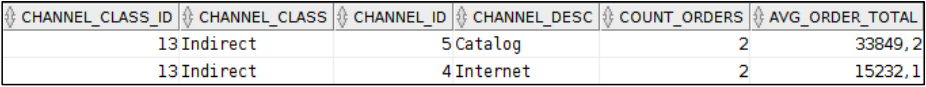
\includegraphics[width=0.85\textwidth]{img//uebung_02_-_aufgabe_02.png}
  \label{img:uebung_02_-_aufgabe_02}
  \caption{Table Function}{CHANNEL\_CLASS\_ID = 13}
\end{figure}


\subsubsection*{Lösung}
\label{sec:uebung_02.aufgabe_02.loesung}
\inputsql{./loesungen/uebung_02/uebung_02_-_aufgabe_02.sql}


% ##########################################################################
% ############################### Aufgabe 03 ###############################
% ##########################################################################
\subsection{Aufgabe - Table Function}
\label{sec:uebung_02.aufgabe_03}
Schreiben Sie eine Table Function, der eine Referenz auf einen Cursor übergeben wird. Dieser soll Kundendatensätze beinhalten und es soll für jeden übergebenen Datensatz der Name des Kunden, sein Land und der durch ihn generierte Umsatz in einer Collection zurückgegeben werden.

Ein exemplarischer Aufruf der Funktion könnte dabei wie folgt aussehen:
\begin{sqlcode}
SELECT *
FROM TABLE(
  tf_customer(
    CURSOR(
      SELECT *
      FROM customers
      WHERE customer_id < 200
    )
  )
);
\end{sqlcode}

Rückgabe bei Aufruf der Table Funktion:
\begin{figure}[H]
  \centering
  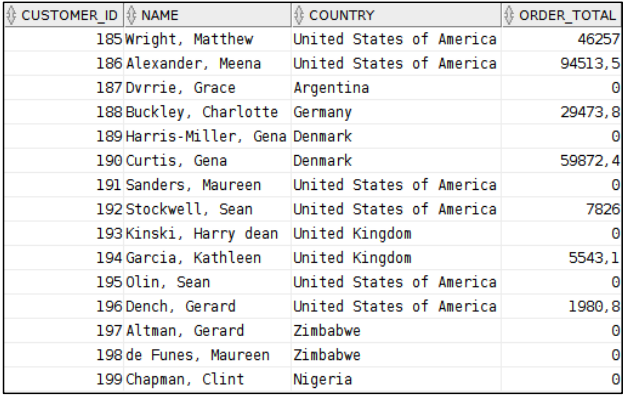
\includegraphics[width=0.75\textwidth]{img//uebung_02_-_aufgabe_03.png}
  \label{img:uebung_02_-_aufgabe_03}
  \caption{Rückgabe}{Rückgabe bei Aufruf der Table Function}
\end{figure}

\subsubsection*{Lösung}
\label{sec:uebung_02.aufgabe_03.loesung}
\inputsql{./loesungen/uebung_02/uebung_02_-_aufgabe_03.sql}


% ##########################################################################
% ############################### Aufgabe 04 ###############################
% ##########################################################################
\subsection{Aufgabe - Pipelined Table Function}
\label{sec:uebung_02.aufgabe_04}
Ändern Sie die Funktion aus Aufgabe \ref{sec:uebung_02.aufgabe_03} so ab, dass es sich um eine Pipelined Table Function handelt.

\subsubsection*{Lösung}
\label{sec:uebung_02.aufgabe_04.loesung}
\inputsql{./loesungen/uebung_02/uebung_02_-_aufgabe_04.sql}


% ##########################################################################
% ############################### Aufgabe 05 ###############################
% ##########################################################################
\subsection{Aufgabe - Procedure}
\label{sec:uebung_02.aufgabe_05}
Schreiben Sie eine Prozedur, die für jede Tabelle in Ihrem Schema eine Kopie mit dem Präfix „tmp\_“ anlegt.

Hinweis: Die View USER\_TABLES listet alle eigenen Tabellen und eine Tabellenkopie kann mit folgendem DDL-Statement erzeugt werden:
\begin{sqlcode}
CREATE TABLE tmp_tabname AS
  SELECT *
  FROM tabname;
\end{sqlcode}

\subsubsection*{Lösung}
\label{sec:uebung_02.aufgabe_05.loesung}
\inputsql{./loesungen/uebung_02/uebung_02_-_aufgabe_05.sql}


% ##########################################################################
% ############################### Aufgabe 06 ###############################
% ##########################################################################
\subsection{Aufgabe - Procedure}
\label{sec:uebung_02.aufgabe_06}
Erzeugen Sie eine weitere Prozedur, die ein Pattern (z.B. '\%A\%') über einen Eingabeparameter erwartet und alle Tabellen löscht, deren Name dem übergebenen Pattern entspricht. Verwenden Sie BIND Variablen wo es möglich ist.

\subsubsection*{Lösung}
\label{sec:uebung_02.aufgabe_06.loesung}
\inputsql{./loesungen/uebung_02/uebung_02_-_aufgabe_06.sql}

  \section{Übung - Modellierung}
\label{sec:uebung_03}
Entwickeln Sie auf Basis des folgenden Schemas einen Entwurf für ein Data Warehouse. Verwenden Sie dazu den Oracle Data Modeler und erzeugen Sie im ersten Schritt ein logisches Modell um anschließend daraus ein relationales Star- und ein relationales Snowflake-Modell entwickeln zu lassen. Lassen Sie sich die DDL-Statements zur Erzeugung der modellierten Tabellen ausgeben.

\begin{figure}[H]
  \centering
  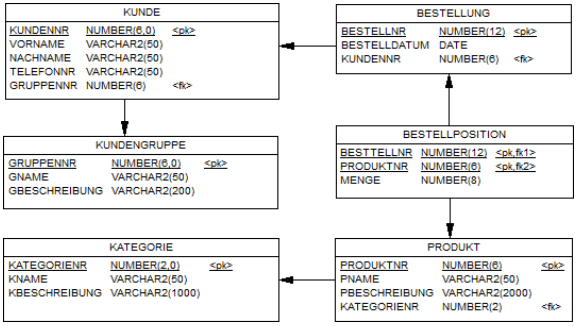
\includegraphics[width=0.85\textwidth]{img//uebung_03_-_schema.png}
  \label{img:uebung_03_-_schema}
  \caption{Schema}
\end{figure} 

Verwenden Sie folgende Leitfragen zur Identifizierung der Granularität und Dimensionen:
\begin{itemize}
  \item Wie viele Produkte wurden 2014 an den Kunden mit der Kundennummer 123 verkauft?
  \item In welcher Kundengruppe wurden im Januar 2015 die meisten Produkte abgesetzt?
  \item Wie oft wurde das Produkt „Ebook-Reader ABC“ am 03.01.2013 verkauft.
  \item Wie viele Produkte der Kategorie „Online-Medien“ wurden am 03.03.2013 um 00:11 verkauft?
  \item In welcher Stunde wurden am 01.01.2016 die meisten Produkte der Produktkategorie **Printmedien** abgesetzt?
  \item Wie viele Produkte der Produktkategorie „Printmedien“ wurden vormittags am 04.02.2013 abgesetzt?
\end{itemize}
  \section{Übung - SCD}
\label{sec:uebung_04}
Gegeben sei folgender Aussschnitt aus einem bestehenden DWH:

Faktentabelle:



% ##########################################################################
% ############################### Aufgabe 01 ###############################
% ##########################################################################
%\label{subsec:uebung_04.aufgabe_01}
%\subsection{Aufgabe}
%
%\subsubsection*{Lösung}
%\label{subsubsec:uebung_04.aufgabe_01.loesung}
%\inputsql{./sql/uebung_04/uebung_04_-_aufgabe_01.sql}

  \section{Übung - Implementierung}
\label{sec:uebung_05}

% ##########################################################################
% ############################### Aufgabe 01 ###############################
% ##########################################################################
\subsection{Aufgabe}
\label{sec:uebung_05.aufgabe_01}
Sie sind beteiligt an der Implementierung eines Core Data Warehouse nach dem Star Schema auf Grundlage der Tabellen des DWH-Users. Alle Core DWH Tabellen sind bereits angelegt, mit Ausnahme der Customer Dimension und der Faktentabelle.

Führen Sie das Skript 04.2-Implementierung\_Skript.sql aus dem Vorlesungsverzeichnis aus, um die notwendige Tabellenstruktur in Ihrem Schema bereit zu stellen und legen Sie anschließend alle fehlenden Tabellen, Constraints usw. an. Letztlich sollen die von Ihnen erstellten Tabellen gefüllt werden. Greifen Sie dazu auf die OLTP-Tabellen aus dem Quellsystem zu.

\subsubsection*{Lösung}
\label{sec:uebung_05.aufgabe_01.loesung}
\inputsql{./loesungen/uebung_05/uebung_05_-_aufgabe_01.sql}

% ##########################################################################
% ############################### Aufgabe 02 ###############################
% ##########################################################################
\subsection{Aufgabe}
\label{sec:uebung_05.aufgabe_02}
Die Vertriebsabteilung benötigt einen stets aktuellen Report, der den Absatz je Produktunterkategorie für jedes Jahr, Quartal und Mitarbeiter ausgibt. Die Datenbasis des Reports soll als eigene Tabelle implementiert werden.

Nutzen Sie hierzu Ihr komplettiertes Core Date Warehouse aus Aufgabe 1. Alternativ können Sie auch auf die Tabellen des DWH's Schemas zugreifen.

\subsubsection*{Lösung}
\label{sec:uebung_05.aufgabe_02.loesung}
\inputsql{./loesungen/uebung_05/uebung_05_-_aufgabe_02.sql}

% ##########################################################################
% ############################### Aufgabe 03 ###############################
% ##########################################################################
\subsection{Aufgabe}
\label{sec:uebung_05.aufgabe_03}
Die Antwortzeiten der folgenden Abfragen sind zu hoch. Erstellen Sie eine geeignete Materialized View. Die Abfragen sollen dabei nicht verändert werden. (Sie müssen die entsprechenden Tabellennamen / Attributsnamen natürlich an Ihr Schema anpassen.)

\subsubsection*{Lösung}
\label{sec:uebung_05.aufgabe_03.loesung}
\inputsql{./loesungen/uebung_05/uebung_05_-_aufgabe_03.sql}

  \section{Übung - OLAP}
\label{sec:uebung_06}

% ##########################################################################
% ############################### Aufgabe 01 ###############################
% ##########################################################################
\label{subsec:uebung_06.aufgabe_01}
\subsection{Aufgabe}
Erzeuge folgende Übersicht über die Anzahl der Mitarbeiter in jeder Abteilung, in jeder Stadt und in jedem Land.

\begin{figure}[H]
  \centering
  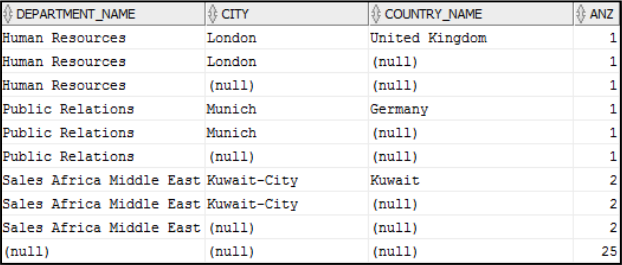
\includegraphics[width=1\textwidth]{img//uebung_06_-_aufgabe_01.png}
  \label{img:uebung_06_-_aufgabe_01}
\end{figure}

\subsubsection*{Lösung}
\label{subsubsec:uebung_06.aufgabe_01.loesung}
\inputsql{./loesungen/uebung_06/uebung_06_-_aufgabe_01.sql}


% ##########################################################################
% ############################### Aufgabe 02 ###############################
% ##########################################################################
\label{subsec:uebung_06.aufgabe_02}
\subsection{Aufgabe}
Zur Übersicht der Mitarbeitergehälter soll folgende Ausgabe mittels geeigneter Gruppierung erreicht werden.


\begin{table}[H]
  \centering
  \begin{tabular}{|l|l|l|l|l|}
    \hline
    \textbf{CITY}  & \textbf{DEPARTMENT} & \textbf{JOB}         & \textbf{NAME}  & \textbf{SALARY}  \\
    \hline
    London         & Human Resources     & \textit{-all-}       & Susan Mavris   & 6500             \\
    London         & Human Resources     & \textit{-all-}       & \textit{-all-} & 6500             \\
    London         & \textit{-all-}      & \textit{-all-}       & \textit{-all-} & 6500             \\
    Munich         & Public Relations    & \textit{-all-}       & Hermann Baer   & 10000            \\
    Munich         & Public Relations    & \textit{-all-}       & \textit{-all-} & 10000            \\
    Munich         & \textit{-all-}      & \textit{-all-}       & \textit{-all-} & 10000            \\
    Oxford         & Sales Europe        & \textit{-all-}       & David Lee      & 6800             \\
    Oxford         & Sales Europe        & \textit{-all-}       & Lisa Ozer      & 11500            \\
    Oxford         & Sales Europe        & \textit{-all-}       & Amit Banda     & 6200             \\
    Oxford         & Sales Europe        & \textit{-all-}       & Ellen Abel     & 11000            \\
    $[$\dots$]$    & $[$\dots$]$         & $[$\dots$]$          & $[$\dots$]$    & $[$\dots$]$          \\
    \textit{-all-} & \textit{-all-}      & Sales Representative & \textit{-all-} & 1157485          \\
    \textit{-all-} & \textit{-all-}      & Shipping Clerk       & \textit{-all-} & 64300            \\
    \textit{-all-} & \textit{-all-}      & Stock Clerk          & \textit{-all-} & 55700            \\
    \textit{-all-} & \textit{-all-}      & Stock Manager        & \textit{-all-} & 36400            \\
    \textit{-all-} & \textit{-all-}      & \textit{-all-}       & \textit{-all-} & 1598401          \\
    \hline
  \end{tabular}
\end{table}

\subsubsection*{Lösung}
\label{subsubsec:uebung_06.aufgabe_02.loesung}
\inputsql{./loesungen/uebung_06/uebung_06_-_aufgabe_02.sql}


% ##########################################################################
% ############################### Aufgabe 03 ###############################
% ##########################################################################
\label{subsec:uebung_06.aufgabe_03}
\subsection{Aufgabe}
Die Vertriebsabteilung benötigt eine Auswertung über den Umsatz zwischen 2010 und 2012 insgesamt, je Jahr, je Land und Region sowie je Jahr, Land und Region.

\begin{table}[H]
  \centering
  \begin{tabular}{|l|l|l|l|}
    \hline
    \textbf{YEAR} & \textbf{COUNTRY} & \textbf{REGION}        & \textbf{SALES}  \\
    \hline
    2010          & China            & Asia                   & 4892716         \\
    2011          & China            & Asia                   & 3056097         \\
    2012          & China            & Asia                   & 4359027         \\
    2010          & Egypt            & Middle East and Africa & 3866210         \\
    2011          & Egypt            & Middle East and Africa & 4397054         \\
    2012          & Egypt            & Middle East and Africa & 3525384         \\
    $[$\dots$]$   &                  &                        &                 \\
                  & China            & Asia                   & 12307840        \\
                  & Egypt            & Middle East and Africa & 11788648        \\
    $[$\dots$]$   &                  &                        &                 \\
    2010          &                  &                        & 125719979       \\
    2011          &                  &                        & 114614129       \\
    2012          &                  &                        & 124466612       \\
                  &                  &                        & 364800720       \\
    \hline
  \end{tabular}
\end{table}

\subsubsection*{Lösung}
\label{subsubsec:uebung_06.aufgabe_03.loesung}
\inputsql{./loesungen/uebung_06/uebung_06_-_aufgabe_03.sql}


% ##########################################################################
% ############################### Aufgabe 04 ###############################
% ##########################################################################
\label{subsec:uebung_06.aufgabe_04}
\subsection{Aufgabe}
Geben Sie für jeden Job, die Anzahl der Mitarbeiter in den Ländern 'United Kingdom', 'United States of America', 'Germany', 'Kuwait', 'Canada' und 'Singapore' in einer Zeile aus.

\begin{figure}[H]
  \centering
  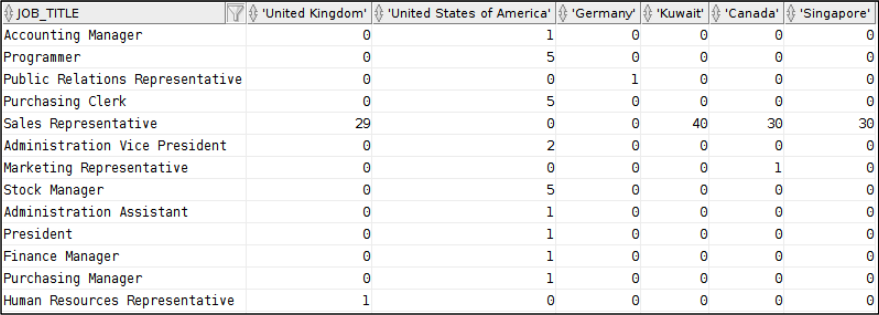
\includegraphics[width=1\textwidth]{img//uebung_06_-_aufgabe_04.png}
  \label{img:uebung_06_-_aufgabe_04}
\end{figure}

\subsubsection*{Lösung}
\label{subsubsec:uebung_06.aufgabe_04.loesung}
\inputsql{./loesungen/uebung_06/uebung_06_-_aufgabe_04.sql}

  \section{Übung - Analytische Funktionen}
\label{sec:uebung_07}

% ##########################################################################
% ############################### Aufgabe 01 ###############################
% ##########################################################################
\subsection{Aufgabe}
\label{subsec:uebung_07.aufgabe_01}
Zeige für jede Bestellposition die insgesamt in der Produktoberkategorie (Parentcategory) abgesetzte Menge.

\begin{figure}[H]
  \centering
  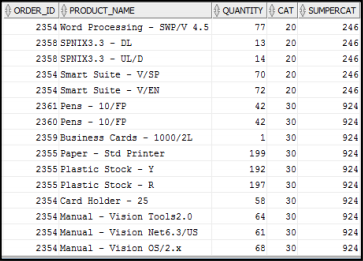
\includegraphics[width=0.8\textwidth]{img//uebung_07_-_aufgabe_01.png}
  \label{img:uebung_07_-_aufgabe_01}
\end{figure}

\subsubsection*{Lösung}
\label{subsubsec:uebung_07.aufgabe_01.loesung}
\inputsql{./loesungen/uebung_07/uebung_07_-_aufgabe_01.sql}


% ##########################################################################
% ############################### Aufgabe 02 ###############################
% ##########################################################################
\subsection{Aufgabe}
\label{subsec:uebung_07.aufgabe_02}
Klassifiziere die Departments nach dem durchschnittlichen Gehalt der Mitarbeiter, die in jenem Department arbeiten, in drei Klassen.

\begin{table}[H]
  \centering
  \ttfamily
  \begin{tabular}{|l|l|l|l|}
    \hline
    \textbf{DEPT\_ID} & \textbf{DEPT\_NAME}  & \textbf{AVG\_SAL} & \textbf{CLASS} \\
    \hline
    140               & Control And Credit   & 0                 & 1              \\
    260               & Recruiting           & 0                 & 1              \\
    150               & Shareholder Services & 0                 & 1              \\
    160               & Benefits             & 0                 & 1              \\
    $[$\dots$]$       &                      &                   &                \\
    20                & Marketing            & 9500              & 3              \\
    70                & Public Relations     & 10000             & 3              \\
    110               & Accounting           & 10154             & 3              \\
    90                & Executive            & 19333,33          & 3              \\
    \hline
  \end{tabular}
\end{table}

\subsubsection*{Lösung}
\label{subsubsec:uebung_07.aufgabe_02.loesung}
\inputsql{./loesungen/uebung_07/uebung_07_-_aufgabe_02.sql}


% ##########################################################################
% ############################### Aufgabe 03 ###############################
% ##########################################################################
\subsection{Aufgabe}
\label{subsec:uebung_07.aufgabe_03}
Welche sind die Top 4 Produktkategorien, gemessen am Umsatz, für alle Bestellungen aus dem Jahr 2014 die an Kunden aus Brasilien gingen?

\begin{table}[H]
  \centering
  \ttfamily
  \begin{tabular}{|l|l|l|l|}
    \hline
    \textbf{P\_CATEGORY\_NAME} & \textbf{CATEGORY\_NAME}  & \textbf{UMSATZ} & \textbf{RANG} \\
    \hline
    hardware & hardware8 & 7228652 & 1 \\
    software & software6 & 7145551 & 2 \\
    hardware & hardware4 & 5216302 & 3 \\
    hardware & hardware3 & 5051191 & 4 \\
    \hline
  \end{tabular}
\end{table}

\subsubsection*{Lösung}
\label{subsubsec:uebung_07.aufgabe_03.loesung}
\inputsql{./loesungen/uebung_07/uebung_07_-_aufgabe_03.sql}


% ##########################################################################
% ############################### Aufgabe 04 ###############################
% ##########################################################################
\subsection{Aufgabe}
\label{subsec:uebung_07.aufgabe_04}
Liste die Umsätze der einzelnen Monate für 2015 auf. Dabei sollen zusätzlich die laufende Summe und der durchschnittliche Umsatz, berechnet aus dem vorherigen, aktuellen sowie nachfolgendem Monat, ausgegeben werden.

\begin{figure}[H]
  \centering
  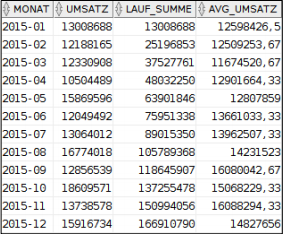
\includegraphics[width=0.6\textwidth]{img//uebung_07_-_aufgabe_04.png}
  \label{img:uebung_07_-_aufgabe_04}
\end{figure}

\subsubsection*{Lösung}
\label{subsubsec:uebung_07.aufgabe_04.loesung}
\inputsql{./loesungen/uebung_07/uebung_07_-_aufgabe_04.sql}


% ##########################################################################
% ############################### Aufgabe 05 ###############################
% ##########################################################################
\subsection{Aufgabe}
\label{subsec:uebung_07.aufgabe_05}
Erzeuge eine Ausgabe mit den Spalten COUNTRY\_NAME, CHANNEL\_DESC, SALES\$, RANG indem für die Vertriebskanäle alle Umsätze, die darüber gemacht wurden von März bis Juni 2008 aufgelistet und in der Spalte RANG den Rang innerhalb der Vertriebskanäle für das jeweilige Land vermerkt ist.

\begin{table}[H]
  \centering
  \ttfamily
  \begin{tabular}{|l|l|l|l|}
    \hline
    \textbf{COUNTRY} & \textbf{CHANNEL\_DESC} & \textbf{SALES\$} & \textbf{RANG}  \\
    \hline
    Argentina        & Direct Sales           & 291299           & 1              \\
    Argentina        & Partners               & 100131           & 2              \\
    Argentina        & Catalog                & 57064            & 3              \\
    Australia        & Tele Sales             & 717783           & 1              \\
    Australia        & Internet               & 508367           & 2              \\
    Australia        & Partners               & 452358           & 3              \\
    Australia        & Catalog                & 175854           & 4              \\
    Australia        & Direct Sales           & 47058            & 5              \\
    Belgium          & Partners               & 661416           & 1              \\
    Belgium          & Catalog                & 448693           & 2              \\
    Belgium          & Direct Sales           & 144147           & 3              \\
    $[$\dots$]$      &                        &                  &                \\
    \hline
  \end{tabular}
\end{table}

\subsubsection*{Lösung}
\label{subsubsec:uebung_07.aufgabe_05.loesung}
\inputsql{./loesungen/uebung_07/uebung_07_-_aufgabe_05.sql}


% ##########################################################################
% ############################### Aufgabe 06 ###############################
% ##########################################################################
\subsection{Aufgabe}
\label{subsec:uebung_07.aufgabe_06}
Welche Produkte wurden häufiger abgesetzt als der Durchschnitt der Produkte innerhalb der jeweiligen Produktoberkategorie (Hardware, Software,…)?

\subsubsection*{Lösung}
\label{subsubsec:uebung_07.aufgabe_06.loesung}
\inputsql{./loesungen/uebung_07/uebung_07_-_aufgabe_06.sql}

  \section{Übung - AWK}
\label{sec:uebung_08}
Die Datei awk\_cust\_awk.csv im Verzeichnis csv hat folgenden Aufbau:

\begin{minted}{bash}
time;first;last;address;custvalue;custorders;id
11:18:40 AM;allyson;dANIELS;2835 Schorsch;1617,39;21;1
6:22:59 AM;LUNA;morse;9627 Pittsburgh;803,25;18;2
9:06:12 PM;Jake;POOLE;6599 Midway Airport;271.46;13;3
\end{minted}

% ##########################################################################
% ############################### Aufgabe 01 ###############################
% ##########################################################################
\subsection{Aufgabe}
\label{sec:uebung_08.aufgabe_01}
Überprüfen Sie die CSV-Datei auf folgende Fehler und schreiben Sie die fehlerhaften Datensätze in eine Datei error\_cust\_data.csv. Beachten Sie dabei, dass in der ersten Zeile Spaltenüberschriften stehen und diese nicht geprüft werden müssen.

\begin{itemize}
\item Jede Zeile enthält genau 7 Felder
\item Die Felder first und last bestehen ausschließlich aus Alphazeichen
\item Die Uhrzeit im Feld time hat folgendes Format: hh:mm:ss AM/PM
  \begin{itemize}
    \item 1 oder 2-stellige Stundenangabe 1-12,
    \item 2 stellige Minuten- und Sekundenangaben 0-59
    \item gefolgt von einem Leerzeichen und AM oder PM
    \item z.B.: 9:18:56 PM oder 11:00:00 AM
  \end{itemize}
\end{itemize}


\subsubsection*{Lösung}
\label{sec:uebung_08.aufgabe_01.loesung}
\inputawk{./loesungen/uebung_08/uebung_08_-_aufgabe_01.awk}


% ##########################################################################
% ############################### Aufgabe 02 ###############################
% ##########################################################################
\subsection{Aufgabe}
\label{sec:uebung_08.aufgabe_02}
Erzeugen Sie mit AWK folgende Ausgabe, bei der die Spaltenüberschrift und die ersten 4 Kunden gefolgt von `………` ausgegeben werden.

Anschließend folgt:
\begin{itemize}
  \item die Anzahl der Kunden
  \item der kleinste Kundenwert
  \item die Anzahl der insgesamt georderten und der durchschnittlich je Kunde georderten Bestellungen
\end{itemize}

\subsubsection*{Lösung}
\label{sec:uebung_08.aufgabe_02.loesung}
\inputawk{./loesungen/uebung_08/uebung_08_-_aufgabe_02.awk}


% ##########################################################################
% ############################### Aufgabe 03 ###############################
% ##########################################################################
\subsection{Aufgabe}
\label{sec:uebung_08.aufgabe_03}
Stellen Sie folgendes sicher (z.B. durch ersetzen der Werte) und überführen Sie die Datei in eine korrigierte CSV-Datei „cust\_bereinigt.csv“, in der alle Felder durch Komma getrennt sind.

\begin{itemize}
  \item Sorgen Sie dafür, dass jeder Vorname und Nachname mit einem Großbuchstaben beginnt und anschließend nur Kleinbuchstaben folgen. (Gehen Sie hier davon aus, dass Vor- und Nachnamen ausschließlich aus Alphazeichen bestehen. Es muss keine Ersetzung eventueller Ziffern oder Sonderzeichen in den Namen durchgeführt werden)
  \item Übertragen Sie die Uhrzeit in das 24 Stunden-Format z. B.: aus `9:08:31 PM` wird `21:08:31` aus `7:45:13 AM` wird `7:45:13`
\end{itemize}


\subsubsection*{Lösung}
\label{sec:uebung_08.aufgabe_03.loesung}
\inputawk{./loesungen/uebung_08/uebung_08_-_aufgabe_03.awk}


% ##########################################################################
% ############################### Aufgabe 04 ###############################
% ##########################################################################
\subsection{Aufgabe}
\label{sec:uebung_08.aufgabe_04}
Bilde folgende Anforderungen durch einen regulären Ausdruck ab:

\begin{itemize}
  \item Eine Postleitzahl soll aus 4 bis 6 Ziffern bestehen, mit der Ziffer 5 beginnen und die letzte Ziffer darf keine 0 sein
  \item Als Größe soll „Large“, „Extra Large“ oder „XX Large“ angegeben werden können.
  \item Durch einen regulären Ausdruck soll sichergestellt werden, dass eine Uhrzeit (24 Stunden, 00 bis 23) im Format hh:mm:ss angegeben wird. Die Angabe der Sekunden soll dabei optional sein.
  \item Das Datum soll in folgendem Format dargestellt werden: dd.mm.yyyy. Der Tag soll dabei zwischen dem 01. und 15 liegen und das Jahr zwischen 1990 und 2010.
\end{itemize}


\subsubsection*{Lösung}
\label{sec:uebung_08.aufgabe_04.loesung}
\inputawk{./loesungen/uebung_08/uebung_08_-_aufgabe_04.awk}



  \section{Übung - External Table}
\label{sec:uebung_09}
In einer CSV Datei (orders.csv) werden Bestelldaten gelistet, die in die Tabellen orders und order\_items aufgenommen werden sollen. Jede Zeile der Datei entspricht einer Bestellposition. Die Datei befindet sich auf dem Server Galway und ist über das Oracle-Directory student\_dir erreichbar.

Dateiaufbau:

\begin{minted}[  linenos,
  autogobble,
  breaklines,]{bash}
order_id;order_date;channel_id;customer_id;order_status; sales_rep_id;product_id;line_item_id;quantity
2362;11.06.2016 17:18:35;9;195;9;104;1781;1;2
2362;11.06.2016 17:18:35;9;195;9;104;1803;2;10
\end{minted}

% ##########################################################################
% ############################### Aufgabe 01 ###############################
% ##########################################################################
\label{subsec:uebung_09.aufgabe_01}
\subsection{Aufgabe}
Definiere eine externe Tabelle für die vorliegende Datei orders.csv.

\subsubsection*{Lösung}
\label{subsubsec:uebung_09.aufgabe_01.loesung}
\inputsql{./loesungen/uebung_09/uebung_09_-_aufgabe_01.sql}


% ##########################################################################
% ############################### Aufgabe 02 ###############################
% ##########################################################################
\label{subsec:uebung_09.aufgabe_02}
\subsection{Aufgabe}
Übertrage mithilfe von zwei INSERT-Statements (INSERT INTO tab\_name SELECT …) alle Daten von der externen Tabelle in die Tabellen orders und order\_items. Als Unit Preis für die bestellten Produkte soll der Listenpreis verwendet werden. ORDER\_TOTAL soll aus der Summe der Einzelpositionen ermittelt werden.

\subsubsection*{Lösung}
\label{subsubsec:uebung_09.aufgabe_02.loesung}
\inputsql{./loesungen/uebung_09/uebung_09_-_aufgabe_02.sql}


% ##########################################################################
% ############################### Aufgabe 03 ###############################
% ##########################################################################
\label{subsec:uebung_09.aufgabe_03}
\subsection{Aufgabe}
Definiere eine externe Tabelle die nur mit der order\_id, channel\_id und dem order\_status der CSV Datei geladen wird.

\subsubsection*{Lösung}
\label{subsubsec:uebung_09.aufgabe_03.loesung}
\inputsql{./loesungen/uebung_09/uebung_09_-_aufgabe_03.sql}

  % Aufzählung aller Bilder
  % \listoffigures

  % Aufzählung aller Tabellen
  % \listoftables

  % Glossary
  \printglossaries

\end{document}
